\documentclass[12pt]{article}
\usepackage[margin=0.8in]{geometry}
\usepackage{amsmath}
\usepackage{amssymb}
\usepackage{xcolor}
\usepackage{tikz}
\usepackage{enumitem}

\title{\LARGE Q3(c): Risk Aversion and Marginal Utility\\Understanding $u'$ is Declining}
\author{ECO 310}
\date{}

\setlength{\parskip}{0.5em}

\begin{document}

\maketitle

\section*{PART 1: FOUNDATIONS}

\subsection*{What is a Utility Function?}

\begin{center}
\colorbox{blue!20}{
\begin{minipage}{0.9\textwidth}
\textbf{Utility Function:} $u(w)$

A mathematical function that represents how much \textbf{satisfaction or happiness} a person gets from having wealth $w$.
\end{minipage}
}
\end{center}

Think of it like a happiness meter:
\begin{itemize}
    \item More wealth $\Rightarrow$ higher utility (you're happier)
    \item But: each extra dollar might not make you \textit{as much} happier as the previous one
\end{itemize}

\subsection*{Example Utility Functions}

\textbf{1. Square Root:} $u(w) = \sqrt{w}$

\begin{itemize}
    \item $w = 100 \Rightarrow u(100) = 10$
    \item $w = 400 \Rightarrow u(400) = 20$
    \item $w = 900 \Rightarrow u(900) = 30$
\end{itemize}

\textbf{2. Logarithm:} $u(w) = \ln(w)$

\begin{itemize}
    \item $w = 10 \Rightarrow u(10) = 2.30$
    \item $w = 100 \Rightarrow u(100) = 4.61$
    \item $w = 1000 \Rightarrow u(1000) = 6.91$
\end{itemize}

\textbf{3. Linear:} $u(w) = w$

\begin{itemize}
    \item $w = 100 \Rightarrow u(100) = 100$
    \item $w = 200 \Rightarrow u(200) = 200$
\end{itemize}

\newpage

\section*{What is Marginal Utility? (Understanding $u'$)}

\begin{center}
\colorbox{green!20}{
\begin{minipage}{0.9\textwidth}
\textbf{Marginal Utility:} $u'(w) = \frac{du}{dw}$

The \textbf{rate of change} of utility with respect to wealth.

\textbf{Translation:} How much does my happiness increase if I get one more dollar?
\end{minipage}
}
\end{center}

\subsection*{Understanding Derivatives Intuitively}

The derivative $u'(w)$ tells you the \textbf{slope} of the utility function at wealth level $w$.

\textbf{High slope (steep):} Each extra dollar gives you a lot more utility

\textbf{Low slope (flat):} Each extra dollar gives you only a little more utility

\subsection*{Example 1: $u(w) = \sqrt{w}$}

Take the derivative:
$$u'(w) = \frac{d}{dw}\sqrt{w} = \frac{1}{2\sqrt{w}}$$

Let's calculate at different wealth levels:

\begin{center}
\begin{tabular}{|c|c|c|}
\hline
\textbf{Wealth $w$} & \textbf{Utility $u(w)$} & \textbf{Marginal Utility $u'(w)$} \\
\hline
$1$ & $1$ & $0.5$ \\
\hline
$100$ & $10$ & $0.05$ \\
\hline
$10000$ & $100$ & $0.005$ \\
\hline
\end{tabular}
\end{center}

\textbf{Key observation:} As wealth increases, marginal utility \textbf{decreases}!

When you're poor ($w=1$), an extra dollar is worth 0.5 units of utility.

When you're rich ($w=10000$), an extra dollar is only worth 0.005 units of utility.

\subsection*{Example 2: $u(w) = \ln(w)$}

Take the derivative:
$$u'(w) = \frac{d}{dw}\ln(w) = \frac{1}{w}$$

\begin{center}
\begin{tabular}{|c|c|c|}
\hline
\textbf{Wealth $w$} & \textbf{Utility $u(w)$} & \textbf{Marginal Utility $u'(w)$} \\
\hline
$1$ & $0$ & $1$ \\
\hline
$10$ & $2.30$ & $0.1$ \\
\hline
$100$ & $4.61$ & $0.01$ \\
\hline
\end{tabular}
\end{center}

Again: marginal utility \textbf{decreases} as wealth increases!

\newpage

\section*{What is the Second Derivative? (Understanding $u''$)}

\begin{center}
\colorbox{red!20}{
\begin{minipage}{0.9\textwidth}
\textbf{Second Derivative:} $u''(w) = \frac{d^2u}{dw^2} = \frac{d(u')}{dw}$

The \textbf{rate of change of marginal utility}.

\textbf{Translation:} How fast is marginal utility decreasing (or increasing)?
\end{minipage}
}
\end{center}

\subsection*{What Does $u''$ Tell Us?}

\textbf{If $u'' < 0$:} Marginal utility is \textbf{decreasing} (utility function curves downward)

This is called \textbf{CONCAVE}

\textbf{If $u'' > 0$:} Marginal utility is \textbf{increasing} (utility function curves upward)

This is called \textbf{CONVEX}

\textbf{If $u'' = 0$:} Marginal utility is \textbf{constant} (utility function is a straight line)

This is called \textbf{LINEAR}

\subsection*{Example: $u(w) = \sqrt{w}$}

First derivative: $u'(w) = \frac{1}{2\sqrt{w}}$

Second derivative:
$$u''(w) = \frac{d}{dw}\left(\frac{1}{2\sqrt{w}}\right) = \frac{d}{dw}\left(\frac{1}{2}w^{-1/2}\right) = -\frac{1}{4}w^{-3/2} = -\frac{1}{4w^{3/2}}$$

\textbf{Notice:} $u''(w) < 0$ for all $w > 0$!

This means marginal utility is always decreasing.

\subsection*{Visual: Concave vs Convex vs Linear}

\begin{center}
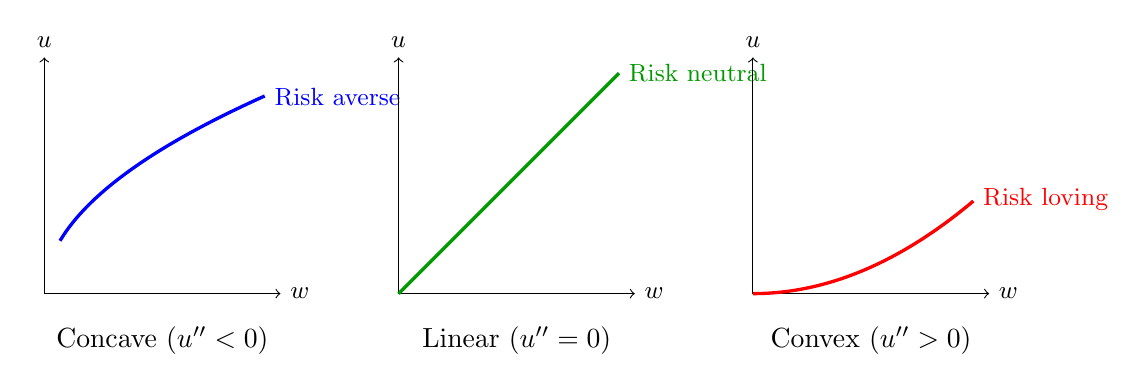
\begin{tikzpicture}[scale=1]
% Concave
\begin{scope}[xshift=0cm]
\draw[->] (0,0) -- (3,0) node[right] {\small $w$};
\draw[->] (0,0) -- (0,3) node[above] {\small $u$};
\draw[very thick, blue, domain=0.2:2.8, smooth, samples=50] plot (\x, {1.5*sqrt(\x)});
\node[below] at (1.5, -0.3) {Concave ($u'' < 0$)};
\node[blue, right] at (2.8, 2.5) {\small Risk averse};
\end{scope}

% Linear
\begin{scope}[xshift=4.5cm]
\draw[->] (0,0) -- (3,0) node[right] {\small $w$};
\draw[->] (0,0) -- (0,3) node[above] {\small $u$};
\draw[very thick, green!60!black] (0,0) -- (2.8, 2.8);
\node[below] at (1.5, -0.3) {Linear ($u'' = 0$)};
\node[green!60!black, right] at (2.8, 2.8) {\small Risk neutral};
\end{scope}

% Convex
\begin{scope}[xshift=9cm]
\draw[->] (0,0) -- (3,0) node[right] {\small $w$};
\draw[->] (0,0) -- (0,3) node[above] {\small $u$};
\draw[very thick, red, domain=0:2.8, smooth, samples=50] plot (\x, {0.15*\x*\x});
\node[below] at (1.5, -0.3) {Convex ($u'' > 0$)};
\node[red, right] at (2.8, 1.2) {\small Risk loving};
\end{scope}
\end{tikzpicture}
\end{center}

\newpage

\section*{What is Risk Aversion?}

\begin{center}
\colorbox{yellow!30}{
\begin{minipage}{0.9\textwidth}
\textbf{Risk Aversion:} A person is risk averse if $u''(w) < 0$

This means: \textbf{They prefer a sure thing over a gamble with the same expected value.}
\end{minipage}
}
\end{center}

\subsection*{Example: Risk Averse Person}

Suppose $u(w) = \sqrt{w}$ and current wealth is $w = 100$.

\textbf{Option A (Sure thing):} Keep \$100 for sure
$$u(100) = \sqrt{100} = 10$$

\textbf{Option B (Gamble):} 50\% chance of \$0, 50\% chance of \$200
$$\text{Expected utility} = 0.5 \cdot u(0) + 0.5 \cdot u(200) = 0.5(0) + 0.5(14.14) = 7.07$$

\textbf{Expected wealth is the same:}
\begin{itemize}
    \item Option A: \$100 for sure
    \item Option B: $0.5(0) + 0.5(200) = \$100$ expected
\end{itemize}

\textbf{But utility is different:}
\begin{itemize}
    \item Option A: $u = 10$
    \item Option B: $u = 7.07$
\end{itemize}

\textbf{Conclusion:} Risk averse person prefers Option A (sure thing) even though both have same expected wealth!

This happens because utility function is \textbf{concave} ($u'' < 0$).

\subsection*{Visual Explanation}

\begin{center}
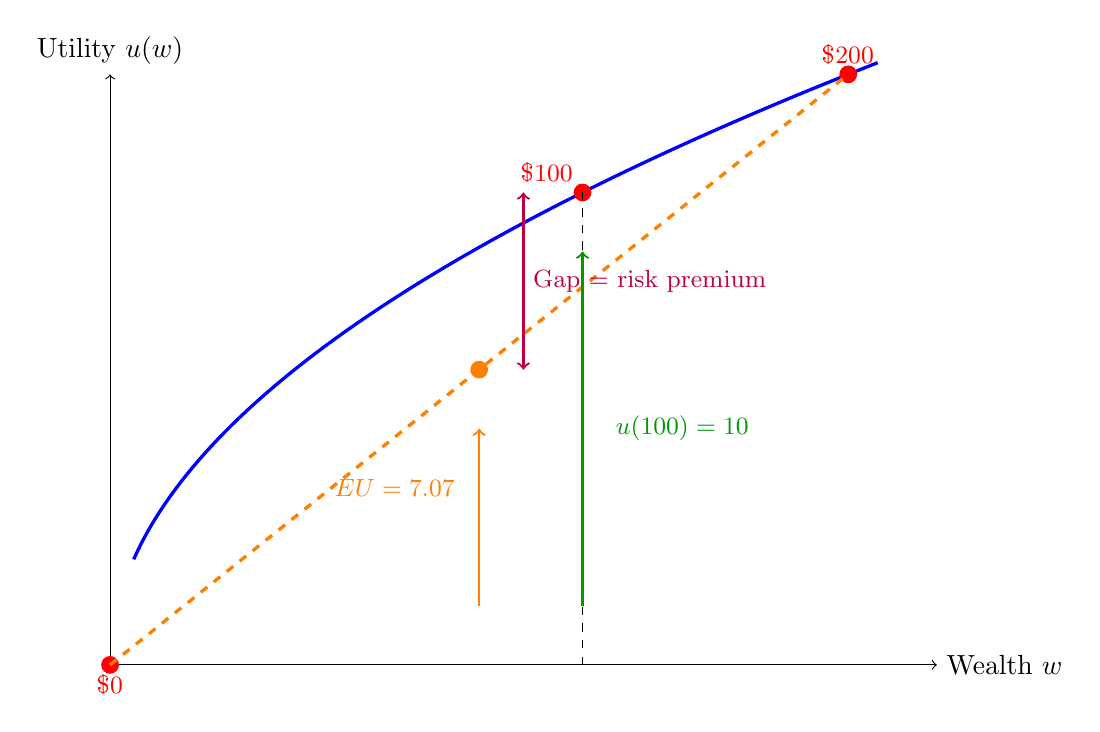
\begin{tikzpicture}[scale=1.5]
% Axes
\draw[->] (0,0) -- (7,0) node[right] {Wealth $w$};
\draw[->] (0,0) -- (0,5) node[above] {Utility $u(w)$};

% Concave utility curve
\draw[very thick, blue, domain=0.2:6.5, smooth, samples=100] plot (\x, {2*sqrt(\x)});

% Mark points
\filldraw[red] (0, 0) circle (2pt) node[below] {\small \$0};
\filldraw[red] (4, 4) circle (2pt) node[above left] {\small \$100};
\filldraw[red] (6.25, 5) circle (2pt) node[above] {\small \$200};

% Draw chord (expected utility of gamble)
\draw[dashed, orange, very thick] (0, 0) -- (6.25, 5);

% Mark expected wealth
\draw[dashed] (4, 0) -- (4, 4);

% Mark utility of sure thing
\draw[->, thick, green!60!black] (4, 0.5) -- (4, 3.5);
\node[green!60!black, right] at (4.2, 2) {\small $u(100) = 10$};

% Mark expected utility of gamble
\filldraw[orange] (3.125, 2.5) circle (2pt);
\draw[->, thick, orange] (3.125, 0.5) -- (3.125, 2);
\node[orange, left] at (3, 1.5) {\small $EU = 7.07$};

% Gap showing risk premium
\draw[<->, thick, purple] (3.5, 2.5) -- (3.5, 4);
\node[purple, right] at (3.5, 3.25) {\small Gap = risk premium};

\end{tikzpicture}
\end{center}

\textbf{Key insight:} The concave curve means the utility of the average is \textbf{higher} than the average of the utilities!

\newpage

\section*{Absolute Risk Aversion (ARA)}

\begin{center}
\colorbox{cyan!20}{
\begin{minipage}{0.9\textwidth}
\textbf{Absolute Risk Aversion (ARA):}
$$A(w) = -\frac{u''(w)}{u'(w)}$$

Measures \textbf{how risk averse} you are in absolute terms.
\end{minipage}
}
\end{center}

\subsection*{What Does ARA Tell Us?}

\textbf{Higher ARA:} More risk averse (avoid risk more)

\textbf{Lower ARA:} Less risk averse (willing to take more risk)

\textbf{Why the negative sign?} Because $u'' < 0$ for risk averse people, so the negative makes $A(w) > 0$.

\subsection*{CARA: Constant Absolute Risk Aversion}

If $A(w)$ is \textbf{constant} (doesn't change with wealth), we call this CARA.

\textbf{Example:} $u(w) = -e^{-\alpha w}$ where $\alpha > 0$

Calculate:
$$u'(w) = \alpha e^{-\alpha w}$$
$$u''(w) = -\alpha^2 e^{-\alpha w}$$
$$A(w) = -\frac{-\alpha^2 e^{-\alpha w}}{\alpha e^{-\alpha w}} = \alpha$$

\textbf{ARA is constant!} No matter your wealth, you have the same absolute risk aversion.

\subsection*{DARA: Decreasing Absolute Risk Aversion}

If $A(w)$ \textbf{decreases} as wealth increases, we call this DARA.

\textbf{Intuition:} As you get richer, you're willing to take more absolute risk (invest more dollars in risky assets).

\textbf{Example:} $u(w) = \sqrt{w}$

Calculate:
$$u'(w) = \frac{1}{2\sqrt{w}}$$
$$u''(w) = -\frac{1}{4w^{3/2}}$$
$$A(w) = -\frac{-\frac{1}{4w^{3/2}}}{\frac{1}{2\sqrt{w}}} = \frac{1}{4w^{3/2}} \cdot \frac{2\sqrt{w}}{1} = \frac{1}{2w}$$

\textbf{As $w$ increases, $A(w)$ decreases!} This is DARA.

\newpage

\section*{Relative Risk Aversion (RRA)}

\begin{center}
\colorbox{magenta!20}{
\begin{minipage}{0.9\textwidth}
\textbf{Relative Risk Aversion (RRA):}
$$R(w) = -\frac{w \cdot u''(w)}{u'(w)} = w \cdot A(w)$$

Measures \textbf{how risk averse} you are in \textbf{relative} (percentage) terms.
\end{minipage}
}
\end{center}

\subsection*{What's the Difference Between ARA and RRA?}

\textbf{Absolute Risk Aversion (ARA):} How many \textbf{dollars} are you willing to risk?

\textbf{Relative Risk Aversion (RRA):} What \textbf{fraction of your wealth} are you willing to risk?

\subsection*{Example: ARA vs RRA}

Suppose you have two people:
\begin{itemize}
    \item Person A: wealth = \$10,000
    \item Person B: wealth = \$1,000,000
\end{itemize}

Both have same RRA = 2, but different ARA.

\textbf{Question:} How much would each invest in a risky asset?

If RRA is constant, they invest the \textbf{same percentage} of wealth:
\begin{itemize}
    \item Person A might invest 50\% = \$5,000
    \item Person B might invest 50\% = \$500,000
\end{itemize}

Even though Person B invests way more \textbf{dollars} (higher absolute risk), they both invest the same \textbf{fraction} of wealth (same relative risk).

\subsection*{CRRA: Constant Relative Risk Aversion}

If $R(w)$ is \textbf{constant}, we call this CRRA.

\textbf{Example:} $u(w) = \frac{w^{1-\gamma}}{1-\gamma}$ where $\gamma > 0$ (and $\gamma \neq 1$)

Calculate:
$$u'(w) = w^{-\gamma}$$
$$u''(w) = -\gamma w^{-\gamma-1}$$
$$R(w) = -\frac{w \cdot (-\gamma w^{-\gamma-1})}{w^{-\gamma}} = \frac{\gamma w^{-\gamma}}{ w^{-\gamma}} = \gamma$$

\textbf{RRA is constant!} No matter your wealth, you invest the same \textbf{fraction} in risky assets.

\subsection*{Special Case: $u(w) = \ln(w)$}

This is CRRA with $\gamma = 1$:
$$u'(w) = \frac{1}{w}$$
$$u''(w) = -\frac{1}{w^2}$$
$$R(w) = -\frac{w \cdot (-1/w^2)}{1/w} = \frac{1/w}{1/w} = 1$$

\textbf{RRA = 1 (constant)}

\newpage

\section*{Summary Table: Risk Aversion Measures}

\begin{center}
\begin{tabular}{|l|l|l|}
\hline
\textbf{Measure} & \textbf{Formula} & \textbf{Interpretation} \\
\hline
Risk aversion & $u''(w) < 0$ & Concave utility, prefer certainty \\
\hline
ARA & $A(w) = -\frac{u''(w)}{u'(w)}$ & Absolute risk aversion \\
\hline
RRA & $R(w) = -\frac{w \cdot u''(w)}{u'(w)}$ & Relative risk aversion \\
\hline
CARA & $A(w) = \text{constant}$ & Same absolute risk at all wealth \\
\hline
DARA & $A'(w) < 0$ & Less absolute risk averse when richer \\
\hline
CRRA & $R(w) = \text{constant}$ & Same \% risk at all wealth \\
\hline
\end{tabular}
\end{center}

\subsection*{Common Utility Functions}

\begin{center}
\begin{tabular}{|l|l|l|l|}
\hline
\textbf{Function} & \textbf{$u(w)$} & \textbf{ARA} & \textbf{RRA} \\
\hline
Logarithmic & $\ln(w)$ & $\frac{1}{w}$ (DARA) & $1$ (CRRA) \\
\hline
Power & $\frac{w^{1-\gamma}}{1-\gamma}$ & $\frac{\gamma}{w}$ (DARA) & $\gamma$ (CRRA) \\
\hline
Square root & $\sqrt{w}$ & $\frac{1}{2w}$ (DARA) & $\frac{1}{2}$ (CRRA) \\
\hline
Exponential & $-e^{-\alpha w}$ & $\alpha$ (CARA) & $\alpha w$ (IRRA) \\
\hline
Linear & $w$ & $0$ & $0$ (Risk neutral) \\
\hline
\end{tabular}
\end{center}

\textbf{Note:} IRRA = Increasing Relative Risk Aversion

\newpage

\section*{PART 2: APPLICATION TO Q3(c)}

\subsection*{What is Part (c) Asking?}

Q3(c) asks: \textit{``Give an interpretation for why the DM prefers state C to state A when the condition from part (b) holds.''}

From part (b), the condition at an interior optimum is:
$$\frac{u'(w^C)}{u'(w^A)} = \frac{r_1^A - r_2^A}{r_2^C - r_1^C} \qquad (*)$$

The question wants us to interpret: \textbf{When does the DM prefer state C over state A?}

\section*{What Does ``Prefer State C'' Mean?}

The DM prefers state C if they have \textbf{higher wealth} in state C than in state A:
$$w^C > w^A$$

where:
\begin{itemize}
    \item $w^A = w_0 + r_1^A x + r_2^A(100-x)$ (wealth in state A)
    \item $w^C = w_0 + r_1^C x + r_2^C(100-x)$ (wealth in state C)
\end{itemize}

\textbf{Key insight:} More wealth = higher utility (since $u' > 0$).

So: $w^C > w^A \Rightarrow u(w^C) > u(w^A)$

\section*{What Does $u'$ Mean?}

\begin{center}
\colorbox{blue!20}{
\begin{minipage}{0.9\textwidth}
\textbf{Notation:}

$u'(w) = \frac{du}{dw}$ = marginal utility of wealth

This measures: ``How much does utility increase per additional dollar?''
\end{minipage}
}
\end{center}

\subsection*{Example:}

If $u(w) = \sqrt{w}$, then:
$$u'(w) = \frac{1}{2\sqrt{w}}$$

When $w = 100$: $u'(100) = \frac{1}{20} = 0.05$

When $w = 10000$: $u'(10000) = \frac{1}{200} = 0.005$

\textbf{Notice:} As wealth increases, marginal utility \textbf{decreases}.

\newpage

\section*{What Does ``Risk Aversion'' Mean?}

\begin{center}
\colorbox{green!20}{
\begin{minipage}{0.9\textwidth}
\textbf{Risk Aversion $\Leftrightarrow$ $u''(w) < 0$}

The utility function is \textbf{concave} (curves downward).
\end{minipage}
}
\end{center}

\subsection*{Three Key Facts:}

\begin{enumerate}
    \item $u'(w) > 0$ : More wealth is better (increasing function)

    \item $u''(w) < 0$ : Marginal utility is decreasing (concave function)

    \item \textbf{Risk aversion} means: diminishing marginal utility of wealth
\end{enumerate}

\subsection*{What is $u''$?}

$$u''(w) = \frac{d^2u}{dw^2} = \frac{d(u')}{dw}$$

This is the \textbf{rate of change of marginal utility}.

\textbf{If $u'' < 0$:} Then $u'$ is a \textbf{decreasing function} of $w$.

\section*{Visual Explanation of Risk Aversion}

\begin{center}
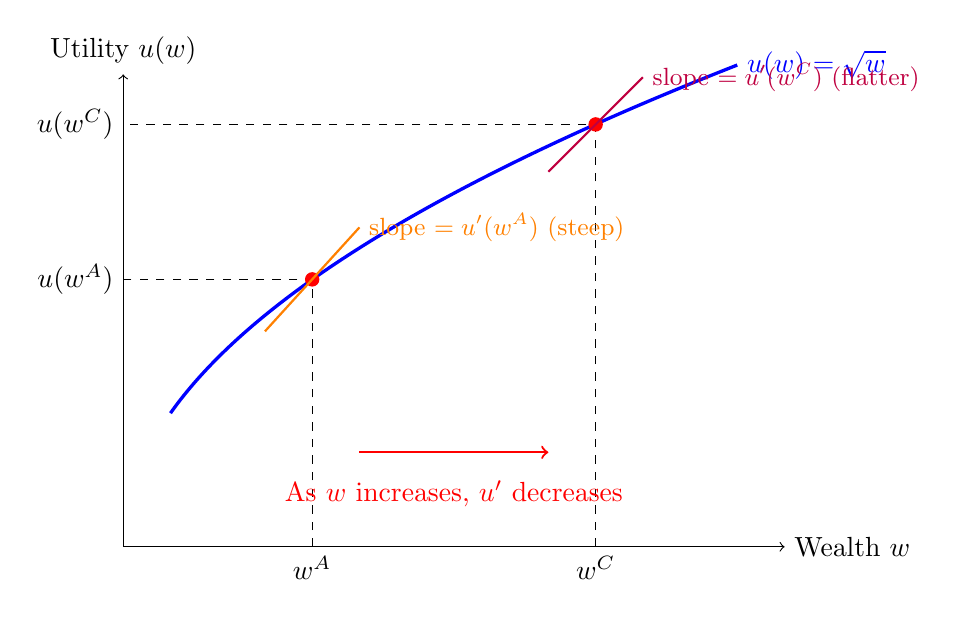
\begin{tikzpicture}[scale=1.2]
% Axes
\draw[->] (0,0) -- (7,0) node[right] {Wealth $w$};
\draw[->] (0,0) -- (0,5) node[above] {Utility $u(w)$};

% Concave utility curve
\draw[very thick, blue, domain=0.5:6.5, smooth, samples=100] plot (\x, {2*sqrt(\x)});
\node[blue, right] at (6.5, 5.1) {$u(w) = \sqrt{w}$};

% Mark two wealth levels
\draw[dashed] (2, 0) -- (2, 2.83) -- (0, 2.83);
\node[below] at (2, 0) {$w^A$};
\node[left] at (0, 2.83) {$u(w^A)$};
\filldraw[red] (2, 2.83) circle (2pt);

\draw[dashed] (5, 0) -- (5, 4.47) -- (0, 4.47);
\node[below] at (5, 0) {$w^C$};
\node[left] at (0, 4.47) {$u(w^C)$};
\filldraw[red] (5, 4.47) circle (2pt);

% Tangent lines showing marginal utility
\draw[thick, orange] (1.5, 2.28) -- (2.5, 3.38);
\node[orange, right] at (2.5, 3.38) {\small slope $= u'(w^A)$ (steep)};

\draw[thick, purple] (4.5, 3.97) -- (5.5, 4.97);
\node[purple, right] at (5.5, 4.97) {\small slope $= u'(w^C)$ (flatter)};

% Arrow showing decreasing slope
\draw[->, thick, red] (2.5, 1) -- (4.5, 1);
\node[red, below] at (3.5, 0.8) {As $w$ increases, $u'$ decreases};

\end{tikzpicture}
\end{center}

\textbf{Key observation:} The slope gets \textbf{flatter} as wealth increases.

$$w^C > w^A \quad \Rightarrow \quad u'(w^C) < u'(w^A)$$

\newpage

\section*{The Logic Chain}

The solution says: ``He prefers state C if $w^C > w^A$; by risk aversion, $u'$ is declining so this holds iff $u'(w^C) < u'(w^A)$.''

Let's break this down:

\subsection*{Step 1: DM prefers state C $\Leftrightarrow$ $w^C > w^A$}

Higher wealth means higher utility (since more money is always better).

\subsection*{Step 2: $w^C > w^A$ $\Leftrightarrow$ $u'(w^C) < u'(w^A)$}

\textbf{Why?} Because of risk aversion ($u'' < 0$), marginal utility is \textbf{declining}.

\begin{center}
\colorbox{yellow!30}{
\begin{minipage}{0.9\textwidth}
\textbf{If and only if (iff):}

$w^C > w^A$ \quad $\Leftrightarrow$ \quad $u'(w^C) < u'(w^A)$

Since $u'$ is a decreasing function, higher wealth means lower marginal utility.
\end{minipage}
}
\end{center}

\subsection*{Step 3: Connect to the FOC}

From part (b), at an interior optimum:
$$\frac{u'(w^C)}{u'(w^A)} = \frac{r_1^A - r_2^A}{r_2^C - r_1^C}$$

Rearranging:
$$u'(w^C) = u'(w^A) \cdot \frac{r_1^A - r_2^A}{r_2^C - r_1^C}$$

\textbf{Question:} When is $u'(w^C) < u'(w^A)$?

\textbf{Answer:} When the multiplier is less than 1:
$$\frac{r_1^A - r_2^A}{r_2^C - r_1^C} < 1$$

This happens when:
$$r_1^A - r_2^A < r_2^C - r_1^C$$

Rearranging:
$$r_1^A + r_1^C < r_2^A + r_2^C$$

\textbf{Interpretation:} State C is preferred when the combined returns from asset 2 exceed the combined returns from asset 1 across states A and C.

\subsection*{Common Confusion: Why Less Than 1, Not Greater Than 1?}

\begin{center}
\colorbox{red!20}{
\begin{minipage}{0.9\textwidth}
\textbf{IMPORTANT:} Students often get the inequality direction backwards!
\end{minipage}
}
\end{center}

\textbf{What we want:} $u'(w^C) < u'(w^A)$ (state C has lower marginal utility)

\textbf{Step 1:} Divide both sides by $u'(w^A)$ (which is positive):
$$\frac{u'(w^C)}{u'(w^A)} < 1$$

\textbf{Step 2:} From the FOC equation (*):
$$\frac{u'(w^C)}{u'(w^A)} = \frac{r_1^A - r_2^A}{r_2^C - r_1^C}$$

\textbf{Step 3:} Substitute:
$$\frac{r_1^A - r_2^A}{r_2^C - r_1^C} < 1$$

So we need the ratio to be \textbf{LESS than 1}, not greater than 1!

\textbf{Why the confusion?}

You might think: ``higher wealth should mean greater marginal utility'' but that's WRONG!

\textbf{Remember:}
\begin{itemize}
    \item Higher wealth $\Rightarrow$ \textbf{lower} marginal utility (risk aversion!)
    \item If $w^C > w^A$ (prefer state C because richer)
    \item Then $u'(w^C) < u'(w^A)$ (lower marginal utility in richer state)
    \item So the ratio $\frac{u'(w^C)}{u'(w^A)} < 1$ (numerator smaller than denominator)
\end{itemize}

\textbf{Bottom line:}
$$u'(w^C) < u'(w^A) \iff \frac{u'(w^C)}{u'(w^A)} < 1 \iff \frac{r_1^A - r_2^A}{r_2^C - r_1^C} < 1$$

All three inequalities use \textbf{less than ($<$)}, not greater than!

\newpage

\section*{Concrete Example}

Suppose:
\begin{itemize}
    \item $w_0 = 1000$, $x = 50$
    \item State A: $r_1^A = 0.1$, $r_2^A = 0.05$ (asset 1 is better)
    \item State C: $r_1^C = 0.02$, $r_2^C = 0.12$ (asset 2 is better)
\end{itemize}

\subsection*{Calculate Wealth:}

\textbf{State A:}
$$w^A = 1000 + 0.1(50) + 0.05(50) = 1000 + 5 + 2.5 = 1007.5$$

\textbf{State C:}
$$w^C = 1000 + 0.02(50) + 0.12(50) = 1000 + 1 + 6 = 1007$$

In this case: $w^A > w^C$, so the DM prefers state A.

\subsection*{Calculate Marginal Utilities:}

If $u(w) = \sqrt{w}$, then $u'(w) = \frac{1}{2\sqrt{w}}$.

\textbf{State A:}
$$u'(w^A) = u'(1007.5) = \frac{1}{2\sqrt{1007.5}} \approx 0.01576$$

\textbf{State C:}
$$u'(w^C) = u'(1007) = \frac{1}{2\sqrt{1007}} \approx 0.01577$$

\textbf{Notice:} $w^A > w^C$ and $u'(w^A) < u'(w^C)$ $\checkmark$

This confirms: higher wealth $\Rightarrow$ lower marginal utility.

\section*{Why Does This Matter?}

The FOC equation (*) balances:
\begin{itemize}
    \item \textbf{LHS:} $\frac{u'(w^C)}{u'(w^A)}$ = ratio of marginal utilities
    \item \textbf{RHS:} $\frac{r_1^A - r_2^A}{r_2^C - r_1^C}$ = ratio of return differences
\end{itemize}

\textbf{Interpretation:}

The DM adjusts $x$ (investment in asset 1) until:
\begin{itemize}
    \item The marginal benefit of investing more in asset 1 (captured by return differences)
    \item Equals the marginal cost in terms of utility (captured by the ratio of marginal utilities)
\end{itemize}

Risk aversion ($u'$ declining) ensures that:
\begin{itemize}
    \item States with higher wealth have lower marginal utility
    \item The DM values an extra dollar more in low-wealth states
    \item This affects how they balance risk across states
\end{itemize}

\newpage

\section*{Key Formulas Summary}

\begin{center}
\begin{tabular}{|l|l|}
\hline
\textbf{Concept} & \textbf{Formula/Definition} \\
\hline
Marginal utility & $u'(w) = \frac{du}{dw} > 0$ \\
\hline
Risk aversion & $u''(w) = \frac{d^2u}{dw^2} < 0$ \\
\hline
Declining marginal utility & $u''(w) < 0 \Rightarrow u'$ is decreasing \\
\hline
Prefer state C & $w^C > w^A \Leftrightarrow u'(w^C) < u'(w^A)$ \\
\hline
FOC from part (b) & $\displaystyle\frac{u'(w^C)}{u'(w^A)} = \frac{r_1^A - r_2^A}{r_2^C - r_1^C}$ \\
\hline
\end{tabular}
\end{center}

\section*{Common Mistakes}

\begin{enumerate}[leftmargin=2cm, itemsep=1em]
    \item \textbf{Confusing $u'$ with $u$}: $u'$ is the \textit{derivative} of utility, not utility itself.

    \item \textbf{Thinking $u' < 0$}: No! $u' > 0$ always (more money is better). It's $u'' < 0$ that defines risk aversion.

    \item \textbf{Forgetting the direction}: Risk aversion means $u'$ is \textit{decreasing}, so higher wealth $\Rightarrow$ lower $u'$.

    \item \textbf{Not connecting to risk aversion}: The key insight is that risk aversion ($u'' < 0$) is what makes the ``iff'' statement work.
\end{enumerate}

\section*{Key Takeaways}

\begin{enumerate}[leftmargin=2cm, itemsep=1em]
    \item \textbf{$u'$ = marginal utility} (how much utility per extra dollar)

    \item \textbf{$u'' < 0$ = risk aversion} (diminishing marginal utility)

    \item \textbf{Risk aversion makes $u'$ declining:} Higher wealth $\Rightarrow$ lower $u'$

    \item \textbf{Prefer state C when $w^C > w^A$}, which by risk aversion means $u'(w^C) < u'(w^A)$

    \item \textbf{The FOC connects return differences to marginal utility ratios} to determine optimal investment
\end{enumerate}

\end{document}
